%=========================================================================
% sec-intro
%=========================================================================

\section{Introduction}

This document describes the verification strategy being used for the
current CERTUS SoC tapeout on the next CRAFT MPW run. This strategy is a
work-in-progress and is continuing to evolve as we make progress towards
the final tapeout deadline. This document also includes discussion of our
future plans for improving this verification strategy in the later phases
of the program.

%=========================================================================
% fig-toplevel-block-diagram
%=========================================================================

\begin{figure}
  \centering
  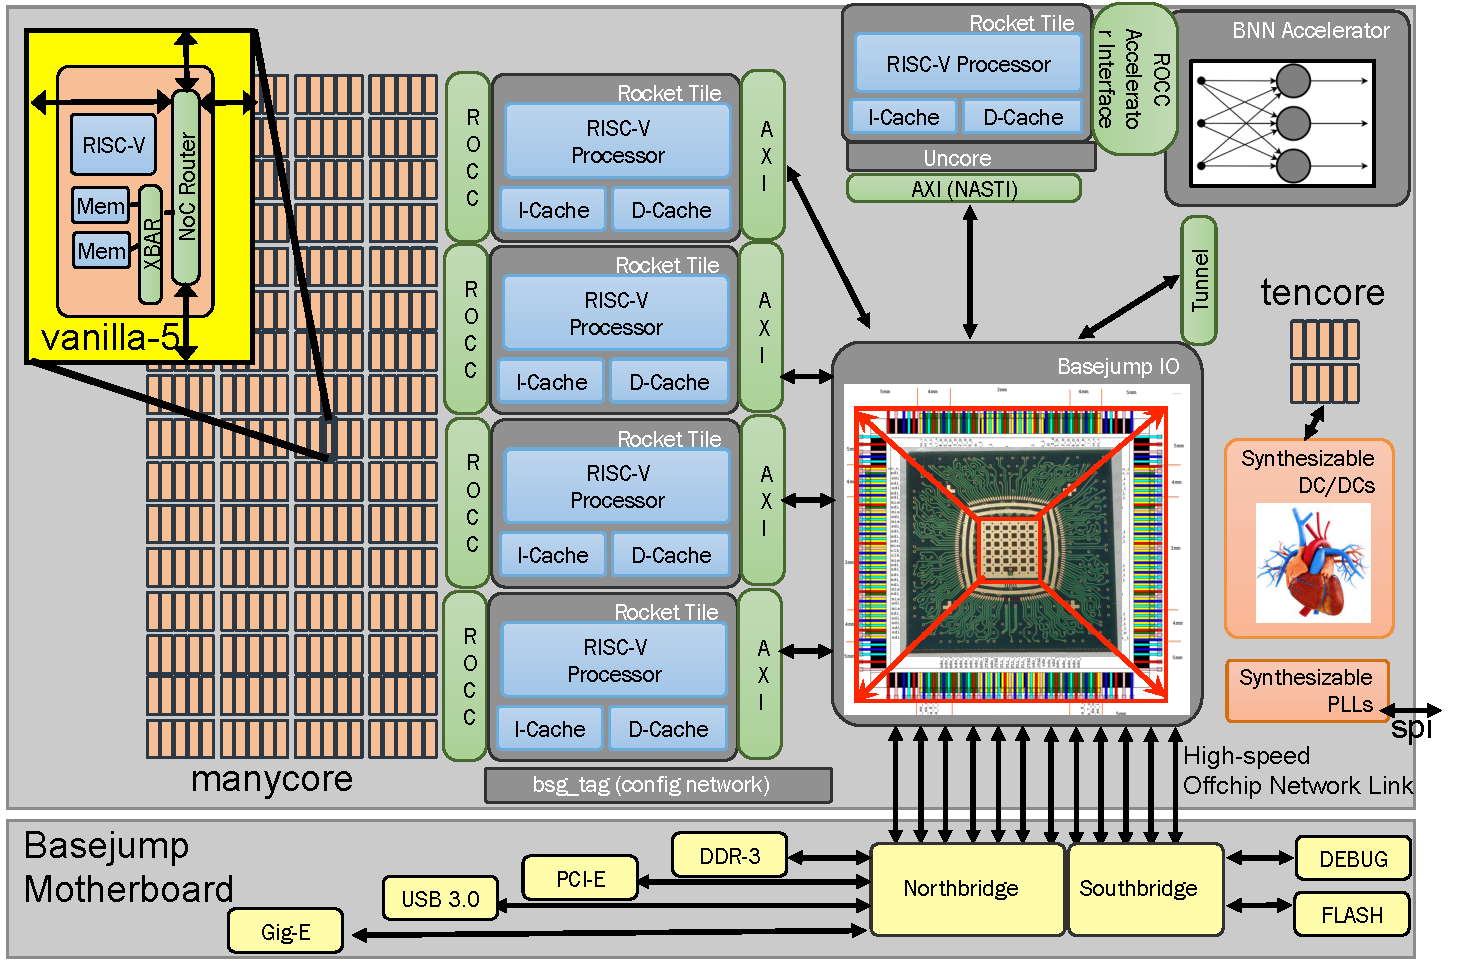
\includegraphics[width=0.9\tw]{toplevel-block-diagram.pdf}
  \caption{\BF{Top-Level Block Diagram for First CERTUS SoC}}
  \label{fig-toplevel-block-diagram}
\end{figure}



Figure~\ref{fig-toplevel-block-diagram} illustrates the top-level block
diagram for the first CERTUS SoC tapeout which includes three key
components: the processor subsystem, accelerator subsystem, and the
mixed-signal subsystem. The \IT{processor subsystem} includes a set of
four RISC-V RV64G Rocket cores each with their own instruction and data
caches. The Rocket cores control a large array of small RISC-V RV32IM
Vanilla-5 cores through the rocket custom coprocessor (RoCC) interface.
Each Vanilla-5 core has its own small instruction and data memory, and
these cores are interconnected through a mesh on-chip network. The cores
communicate to the rest of the chip through the \TT{bsg\_tag} interface
for configuration and through NASTI interfaces (similar to AXI) for
memory management. A smaller ten-core Vanilla-5 array is also included as
a separate part of the processor subsystem; this array serves as a test
vehicle for the digital low-drop-out regulator. The \IT{accelerator
  subsystem} includes a RISC-V RV64G Rocket core which controls a
binarized neural network (BNN) accelerator through the RoCC interface.
Again, the Rocket core communicates to the rest of the chip through the
\TT{bsg\_tag} interface for configuration and through a NASTI interface
for memory management. The \IT{mixed-signal subsystem} includes a
synthesizable phase-locked loop (PLL) to generate various on-chip clock
signals for the entire chip, along with a synthesizable digital
low-drop-out (DLDO) regulator. The PLL and DLDO subsystems are configured
through dedicated off-chip interfaces (either SPI or direct input pins).
These three subsystems are integrated into a full-system via the
\IT{basejump I/O} which includes adapters to convert NASTI interfaces
into a simpler internal message interface and then a centralized bus to
enable the various subsystems to communicate off-chip. Off-chip
communication is via a simple multi-channel source-synchronous protocol
called \TT{bsg\_comm}.

%=========================================================================
% fig-verification-flow
%=========================================================================

\begin{figure}
  \centering
  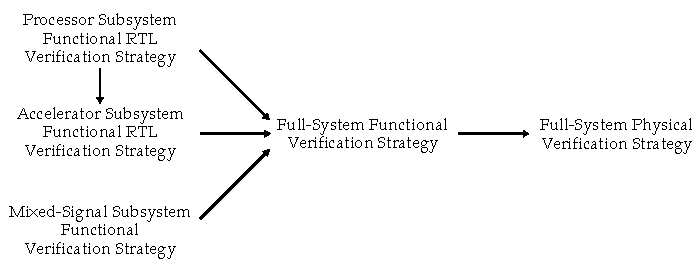
\includegraphics[width=0.8\tw]{verification-flow.svg.pdf}
  \caption{\BF{Overview of CERTUS SoC Verification Strategy}}
  \label{fig-verification-flow}
\end{figure}



Figure~\ref{fig-verification-flow} illustrates the five phases
of our overall verification strategy. Each subsystem is first rigorously
tested in isolation before the subsystems are combined for full-system
functional verification and full-system physical verification.

\medskip
\begin{cbxlist}{1.5em}{1em}{1em}

 \item The \IT{processor subsystem functional RTL verification strategy}
    includes:

    \smallskip
    \begin{cbxlist}[--]{1.5em}{0em}{0em}
      \raggedright

      \item testing BSG library component RTL using directed and random
         unit tests;
      \item testing the on-chip network RTL using directed and random
         tests;

      \item testing single Vanilla-5 core RTL using self-checking
         assembly test programs;

      \item testing the Vanilla-5 ten-core RTL using self-checking
         assembly test programs;

      \item testing the Vanilla-5 manycore RTL using self-checking
         assembly test programs;

      \item testing a single Rocket core RTL using self-checking
         assembly test programs;

      \item testing the Rocket+manycore RTL using self-checking assembly
         test programs;

      \item further testing of the Rocket core RTL using small C test
         programs running \\\hspace{0.5em}on either the bare metal or
         proxy kernel software stacks;

      \item further testing of the Rocket+manycore RTL using small C test
         programs running \\\hspace{0.5em}on either the bare metal or
         proxy kernel software stacks.

    \end{cbxlist}

 \item The \IT{accelerator subsystem functional RTL verification
   strategy} includes:

    \smallskip
    \begin{cbxlist}[--]{1.5em}{0em}{0em}
      \raggedright

      \item validation of algorithm using a high-level description of the
         algorithm to be accelerated;

      \item testing the manually written C++/SystemC implementations of
         the algorithm using the \\\hspace{0.5em}high-level description
         of algorithm as a golden reference;

      \item testing the RTL generated automatically through high-level
         synthesis (HLS) using the \\\hspace{0.5em}C++/SystemC
         implementations as a golden reference;

      \item testing the Rocket+accelerator RTL using self-checking
         assembly test programs;

      \item further testing of the Rocket+accelerator RTL using small C
         test programs running \\\hspace{0.5em}on either the bare metal
         or proxy kernel software stacks;

      \item testing complete end-to-end workload scenarios.

    \end{cbxlist}

 \item The \IT{mixed-signal subsystem functional verification} includes:

    \smallskip
    \begin{cbxlist}[--]{1.5em}{0em}{0em}
      \raggedright

      \item validating the PLL using a system-level model;

      \item testing the PLL RTL and gate-level models using system-level
         model as a golden reference;

      \item testing the PLL extracted transistor-level models using
         system-level model as a golden reference;

      \item testing the DLDO custom cell transistor-level models using
         directed unit tests;

      \item testing the DLDO RTL and gate-level models using directed
         unit tests;

      \item testing the DLDO extracted transistor-level models using
         directed unit tests;

      \item using DLDO post-silicon configuration to avoid pre-silicon
         verification.

    \end{cbxlist}

 \item The \IT{full-system functional verification strategy} uses the
    concept of iterative ``tape-ins'' towards the final ``tape-out''.
    Each tape-in is an instance of a complete chip, but which only
    implements a subset of the desired final functionality. Tape-ins are
    taken through both functional and physical verification. Each tape-in
    gradually adds more complexity until we converge on the final
    full-system. Each tape-in includes the basejump I/O for communicating
    with the final test board including the \TT{bsg\_comm} and
    \TT{bsg\_tag} interfaces and the actual gateware that will be present
    in the test board's FPGA. Tape-in functional verification is done
    primarily through RTL simulation using either directed tests or
    assembly/C test programs. The set of incremental tape-ins are:

    \smallskip
    \begin{cbxlist}[--]{1.5em}{0em}{0em}
      \raggedright

      \item basejump I/O;
      \item basejump I/O with single Vanilla-5 core;
      \item basejump I/O with Vanilla-5 ten-core;
      \item basejump I/O with single Rocket core;
      \item basejump I/O with Rocket+manycore composition;
      \item basejump I/O with Rocket+accelerator composition;
      \item basejump I/O with Rocket+manycore and Rocket+accelerator composition;
      \item basejump I/O with single Rocket core with the PLL;
      \item basejump I/O with Vanilla-5 ten-core with the DLDO;
      \item basejump I/O with Rocket+manycore, Rocket+accelerator,
         Vanilla-5 ten-core, PLL, DLDO.

    \end{cbxlist}

 \item The \IT{full-system physical verification strategy} takes each
    tape-in through all of the front-end, back-end, and manufacturing
    verification steps including:

    \smallskip
    \begin{cbxlist}[--]{1.5em}{0em}{0em}
      \raggedright

      \item post-synthesis functional gate-level simulation;
      \item post-synthesis back-annotated gate-level simulation;
      \item post-synthesis logical equivalence checking against RTL;
      \item post-pnr functional gate-level simulation;
      \item post-pnr back-annotated gate-level simulation;
      \item post-pnr logical equivalence checking against post-synthesis
         gate-level netlist;
      \item post-pnr connectivity, antenna, timing check;
      \item post-pnr block-level design rule check;
      \item full-chip design rule check;
      \item full-chip layout vs schematic check;
      \item full-chip timing signoff;
      \item full-chip signal integrity signoff;
      \item full-chip IR drop signoff;
      \item full-chip electromigration signoff;
      \item full-chip layout patterning check and shape simulation;
      \item full-chip virtual chemical mechanical polishing check and
         thickness simulation.

    \end{cbxlist}

\end{cbxlist}

\medskip\noindent
In the rest of this document, we go into more depth on each of the
five phases of our overall verification strategy. We also describe our
use of preliminary tape-outs to help verify subsystems, and future plans
for improving this verification strategy as part of phase 2 and 3 of the
program.
